\section{Расчет гороскопа рождения}

Мы не будем утруждать читателя углублением в астрономию, так как об этой области знаний достаточно много написано, а также и потому, что сами по себе знания астрономии вовсе не являются гарантом удачных астрологических предсказаний. Большинство астрологов, практикующих Индийскую предсказательную астрологию, всю рутинную, кропотливую работу, связанную с расчетом гороскопа, доверяют компьютеру, используя для этого специальные программы, а всю мощь своего интеллекта и подсознания направляют на решение чисто астрологических задач --- интерпретацию полученных данных и предсказания.

Древние риши (видящие) использовали для определения судьбы человека 9 планет, 12 знаков Зодиака, 12 домов, 27 лунных созвездий.

9 планет --- Солнце, Луна, Марс, Меркурий, Юпитер, Венера и Сатурн --- это реально существующие небесные тела, а также Раху\footnote{Раху --- восходящий северный узел} и Кету\footnote{Кету --- нисходящий южный узел.}, которые являются математически вычисленными точками пересечения орбит Луны и Земли\footnote{В астрологии названия планет не соответствуют астрономическим понятиям о небесных телах (например, Солнце --- это звезда, Луна --- спутник) --- примеч.\,ред.}

\begin{table}[tph!]
	\caption{Символические обозначения 12 знаков зодиака.}
	\label{tbl:signs}

	\centering

	% Расширить по вертикали
	\renewcommand{\arraystretch}{2}

	% Разширить вширь
	\setlength{\tabcolsep}{.05\textwidth}

	% Заполним данными
	\begin{tabular}{lll}
		\aries\ --- Овен      & \leo\ --- Лев    & \sagittarius\ --- Стрелец \\
		\taurus\ --- Телец    & \virgo\ --- Дева & \capricornus\ --- Козерог \\
		\gemini\ --- Близнецы & \libra\ --- Весы & \aquarius\ --- Водолей \\
		\cancer\ --- Рак      & \scorpio\ --- Скорпион & \pisces\ --- Рыбы \\
	\end{tabular}
\end{table}

\begin{table}[tph!]
	\caption{Принятые в астрологии символы для обозначения планет.}
	\label{tbl:planets}

	\centering

	% Расширить по вертикали
	\renewcommand{\arraystretch}{2}

	% Разширить вширь
	\setlength{\tabcolsep}{.05\textwidth}

	% Заполним данными
	\begin{tabular}{lll}
		\astrosun\ --- Солнце & \mercury\ --- Меркурий & \saturn\ --- Сатурн \\
		\fullmoon\ --- Луна   & \jupiter\ --- Юпитер   & \ascnode\ --- Раху \\
		\mars\ --- Марс       & \venus\ --- Венера     & \descnode\ --- Кету
	\end{tabular}
\end{table}

Для составления гороскопа нужно провести расчет координат 9 планет и восходящего знака Зодиака в момент рождения человека, который включает:
\begin{myitem}
	\item Дату рождения
	\item Точное время рождения
	\item Место рождения
\end{myitem}

Если человек не знает своего точного времени рождения, он может обратиться в родильный дом, где в книге регистрации новорожденных данные о времени рождения хранятся в течение 75 лет.

Если у вас нет специальной компьютерной программы, то для расчета необходимо также иметь следующую литературу:
\begin{myenum}
	\item Эфемериды --- астрономические таблицы, по которым определяются положения планет в знаках зодиака в момент рождения.
	\item Таблицы домов Плацидуса (или Коха) для определения координат восходящего знака Зодиака в момент рождения.
	\item Справочник ``Координаты городов и изменения исчисления времени на территории СССР с 1917 по 1992 год''. (Воронеж,\,1992)
\end{myenum}

Эфемериды и таблицы домов Плацидуса (или Коха) можно приобрести в розничной книжной торговле или взять в библиотеке.

Двенадцатью домами гороскопа определяется характер, поведение, способности человека и его судьба. Каждый дом гороскопа отвечает за ту или иную сферу человеческой жизни, то есть представляет различные идеи:

\begin{myenum}
	\item \textbf{Первый дом:}
		\begin{mydescr}
			\item[Физиология] --- голова, мозг.
			\item[Идеи] --- Личность, характер, эго, темперамент, физическое тело, внешний вид, опасности для тела, жизнестойкость, сохранение жизни и здоровья, поведение и привычки, патриотизм, родина, физическая сила, ум, счастье и горе.
		\end{mydescr}
	\item \textbf{Второй дом:}
		\begin{mydescr}
			\item[Физиология] --- правый глаз, лицо, зубы, шея
			\item[Идеи] --- Богатство, деньги, финансовые дела, драгоценные камни и металлы, семья и семейные дела, платежеспособность, обеспеченность, иждивенцы, все члены семьи, торговля, купля-продажа, обмен, процесс еды, пища, диета, речь, движимое имущество.
		\end{mydescr}
	\item \textbf{Третий дом:}
		\begin{mydescr}
			\item[Физиология] --- руки, правое ухо, плечи, кисти.
			\item[Идеи] --- Братья и сестры, средства информации и связи, смелость, мужество, младшие брат и сестра, военная сила, армия, оружие, слуга, союзник, почерк, мастерство рук, путешествия на короткие расстояния, смерть родителей.
		\end{mydescr}
	\item \textbf{Четвертый дом:}
		\begin{mydescr}
			\item[Физиология] --- грудь, сердце, легкие.
			\item[Идеи] --- Дом, квартира, недвижимость, земельный участок, мать, друзья, дружелюбие, все продукты земли, все транспортные средства (автомобиль, аэроплан и\,т.\,п.), перевозка и доставка, удовольствия и комфорт, могила, яма, доверие, родственники.
		\end{mydescr}
	\item \textbf{Пятый дом:}
		\begin{mydescr}
			\item[Физиология] --- желудок, печень, почки, матка, беременность. 
			\item[Идеи] --- Дети, образование, интеллект, знания, умственные способности, наука, ученость, последователи, советы, проницательность, сообразительность, моральные устои, предусмотрительность, мантры, практика йоги, любовные дела, политическая мудрость.
		\end{mydescr}
	\item \textbf{Шестой дом:}
		\begin{mydescr}
			\item[Физиология] --- область пупка, кишечник.
			\item[Идеи] --- Болезни, несчастные случаи, враг, недоброжелатель, жестокие дела и поступки, вражда, рана, опухоль, шрам, свищ, абсцесс, язва, ссоры, спорт, тревоги и беспокойства, страх, горе, недоверие, подозрение, дядя по матери, препятствия, воры, долги.
		\end{mydescr}
	\item \textbf{Седьмой дом:}
		\begin{mydescr}
			\item[Физиология] --- мочевой пузырь, область под пупком.
			\item[Идеи] --- Супружеские отношения, брак, сексуальные удовольствия, поездки, отъезды и приезды, общественные дела, желания, коммерческая деятельность, торговля, бизнес, выигрыш в азартной игре, муж и жена, любовник и любовница, сделка.
		\end{mydescr}
	\item \textbf{Восьмой дом:}
		\begin{mydescr}
			\item[Физиология] --- Половые органы, выделительная система.
			\item[Идеи] --- Смерть, долговечность, потеря, утрата, разрушение, смертоносное оружие, сумасшедший дом, опасность и риск, вина, порок, зло, клевета, критическое состояние, несчастный случай, бедствие, исчезновение, дезертирство, судебный процесс, обвинение, оскорбление, несправедливость, тайные дела, секрет, нарушение обычаев, психические силы, джйотиш, способность предсказывать, задержание, конспирация, изгнание, наследство, разрыв союза, сражения, насильственная смерть.
		\end{mydescr}
	\item \textbf{Девятый дом:}
		\begin{mydescr}
			\item[Физиология] --- бедра.
			\item[Идеи] --- Отец, религия, судьба, удачи и неудачи, религиозные организации, обращение в какую-то веру, добродетель, начальники, духовные наставники, путешествия, братья жены и мужа, священники, паломничество, честность, чистота, право, справедливое решение, внуки, лекарства, богатство, изобилие.
		\end{mydescr}
	\item \textbf{Десятый дом:}
		\begin{mydescr}
			\item[Физиология] --- колени.
			\item[Идеи] --- Карьера, занятие, работа, деятельность, профессия, должность, призвание, отец, правительство, покровительство, защита, известность, слава, почет, уважение, репутация, государственные функции, власть, конференции, печать полномочий, общественное положение.
		\end{mydescr}
	\item \textbf{Одиннадцатый дом:}
		\begin{mydescr}
			\item[Физиология] --- икры ног, лодыжки, левое ухо.
			\item[Идеи] --- Доходы и прибыли, приобретения, выигрыш, старшие братья и сестры, заработки, различные украшения, надежды и их осуществление, дети одного из супругов от других браков, процветание, друзья, домашние животные.
		\end{mydescr}
	\item \textbf{Двенадцатый дом:}
		\begin{mydescr}
			\item[Физиология] --- стопы, левый глаз.
			\item[Идеи] --- Потеря, тяжелая утрата, уменьшение чего-либо, конфискация, длительные зарубежные путешествия, просветление, отделение, больница, тюрьма, монастырь, казарма, растраты, благотворительные действия, дядя и тетя по отцу, грехи.
		\end{mydescr}
\end{myenum}

Двенадцать домов гороскопа разделены на следующие группы:
\begin{myitem}
	\item 1,\,4,\,7\,и\,10-й дома --- кендры, или квадранты (благоприятные)
	\item 1,\,5,\,и\,9-й дома --- тригон (благоприятные)
	\item 6,\,8,\,и\,12-й дома --- неблагоприятные
	\item 3,\,6,\,10,\и\,11-й дома --- дома роста (если неблагоприятные по своей природе планеты находятся в данных домах, то сила этих планет и домов возрастает с каждым годом).
\end{myitem}

\emph{Примечание} --- 6-й дом является одновременно неблаготворным домом и домом роста, то есть значения естественно неблаготворных --- улучшаются. 10-й дом является одновременно домом кендр и домом роста и поэтому любая планета в нем даст положительный результат. 2-й дом --- нейтральный.

Когда Юпитер, Венера, Луна и Меркурий находятся в домах кендр и тригона, они влияют благотворно. Когда эти планеты в 6,\,8,\,и\,12-м домах, то человека преследуют неудачи.

Марс, Солнце, Сатурн, Раху и Кету, находясь в домах кендр и тригона, будут действовать по-разному в зависимости от знака Зодиака, в котором они будут расположены.

Присутствие Солнца, Марса, Сатурна, Раху и Кету в 8-м и 12-м домах окажет неблагоприятное воздействие на жизнь человека. Но если эти планеты будут находиться под влиянием естественно благотворных планет, то зло их уменьшится.

Как планеты воздействуют на жизнь человека в определенных знаках и домах, вы узнаете из следующих глав этой книги.

\subsection{Расчет координат восходящего знака (Asc)}

Наша планета вращается не только вокруг Солнца, но и вокруг своей оси, что является причиной смены дня и ночи. Для удобства измерения времени и пространства Земля разделена на 360 условных линий --- долгот. Полный оборот вокруг своей оси Земля делает за 24 часа, или 1440 минут. Если разделить 1440 минут на 360, мы получим 4 минуты --- время поворота Земли на \(1^\circ\), или время прохождения Солнца между долготами.

Восходящий знак --- это одно из созвездий Зодиака, которое появляется на восточном горизонте в момент рождения человека. Расчет координат восходящего знака --- это расчет координат точки эклиптики на восточном горизонте в момент рождения. Точка назвается \emph{асцедент} и обозначается в эфемеридах --- \emph{Asc}. Необходимо знать, что каждый знак Зодиака занимает \(30^\circ\) пространства. Всего в гороскопе 12 знаков: \(12 * 30^\circ = 360^\circ\) --- полный Зодиак.

Асцендент проходит через \(360^\circ\) полного Зодиака за 24 часа.

Теперь мы можем начать расчет асцендента на нашем примере. Вначале необходимо определить сидерическое(звездное) время в момент рождения человека. В эфемеридах оно указано для каждого дня в 0 часов по Гринвичу и обозначается \emph{Sid Time}.

Откроем эфемериды на странице, где указано сидерическое время для 4 и 5 декабря 1957 года, и выпишем его значения:

\begin{mylist}
	\item 4 декабря 1957 года Sid. Time = \timeshort{4}{50}{10}
	\item 5 декабря 1957 года Sid. Time = \timeshort{4}{54}{7}
\end{mylist}

Далее, решая пропорцию, определяем звездное время в момент рождения(\timeshort{9}{35}{}) по Гринвичу:

\calc{\dfrac{4:54:07 - 4:50:10}{24} * 9:35 + 4:50:10 = 4:51:44}

Теперь требуется определить географические координаты города Харькова. Еще раз возьмем известный нам справочник и на странице 32 найдем Харьков. Выпишем координаты, соответствующие месту нахождения города:

\begin{mylist}
	\item северная широта --- \coord{50}{00}{00}
	\item восточная долгота --- \coord{36}{15}{00}
\end{mylist}

Если нет справочника, определим географические координаты города Харькова по атласу.

Переведем долготу во время путем деления на 15. Это связано с тем, что скорость вращения Земли равна \(15^\circ\) долготы в час. Теперь у нас есть три величины времени:

\begin{mylist}
	\item время рождения --- \timeshort{9}{35}{}
	\item звездное время --- \timeshort{4}{51}{44}
	\item долготное время --- \timeshort{2}{25}{}
\end{mylist}

Так как Харьков находится в восточном полушарии, то сложим эти три величины времени:

\calc{9:35 + 4:51:44 + 2:25 = 16:51:44}

Полученный результат является окончательным звездным временем. Используя таблицы домов Плацидуса (или Коха) найдем звездную величину \timeshort{16}{51}{44} в графе \emph{Sid. Time}. В таблице домов величина \timeshort{16}{51}{44} находится между двух других величин звездного времени --- \timeshort{16}{50}{34} и \timeshort{16}{54}{53}. Напротив первого звездного времени на широте \(50^\circ\) в графе \emph{Asc} вы увидите данные \(23^\circ\)\aquarius\(23^\prime\) (напомним: \aquarius --- Водолей), а напротив другоо звездного времени на той же широте в графе \emph{Asc} будут другие данные: \(25^\circ\)\aquarius\(24^\prime\). В таблице домов Плацидуса это выглядит так:

 
\begin{table}[tph!]
	\centering

	% Расширить по вертикали
	\renewcommand{\arraystretch}{1.5}

	% Заполним данными
	\begin{tabular}{|c|c|c|c|}
		\hline
		\emph{Sid. Time}  & Lat \(49^\circ\) \emph{Asc} & Lat \(50^\circ\) \emph{Asc} & Lat \(51^\circ\) \emph{Asc} \\
		\hline
		\calc{16 - 50 - 34} & \(24^\circ\)\aquarius\(29^\prime\) & \(23^\circ\)\aquarius\(23^\prime\) & \(22^\circ\)\aquarius\(11^\prime\) \\
		\calc{16 - 54 - 53} & \(26^\circ\)\aquarius\(28^\prime\) & \(25^\circ\)\aquarius\(24^\prime\) & \(24^\circ\)\aquarius\(14^\prime\) \\
		\hline
	\end{tabular}
\end{table}

\begin{myenum}
	\item Определим разницу между двумя звездными величинами, указанными в таблице(в минутах):
		\calc{16:54:53 - 16:50:34 = 4:19:00 = 4.316}
	\item Определим разницу между окончательной звездной величной (\timeshort{16}{51}{44}) и первой звездной величиной, указанной в таблице (\timeshort{16}{50}{34})(в минутах):
		\calc{16:51:44 - 16:50:34 = 00:01:10 = 1.16}
	\item Определим разницу между двумя величинами, которые указаны в графе \emph{Asc} на широте \(50^\circ\) (Lat. \(\50^\circ\) (в минутах):
		\calc{\(25^\circ\)\aquarius\(24^\prime\) - \(23^\circ\)\aquarius\(23^\prime\) = \coord{2}{1}{0} = 2.016}
	\item Определим асцендент. \coord{23}{23}{00} можно записать как 23,383\(^\circ\):
		\calc{\dfrac{2.016}{4.316} * 1.16 + 23.383 = 23.924834} или \coord{23}{55}{29} Водолея
	\item Вычитаем величину уже известной нам аянамсы:
		\calc{\coord{23}{55}{29} - \coord{23}{16}{21} = \coord{00}{39}{08}}
\end{myenum}

Итак, асцендент равен \coord{00}{39}{08} Водолея. На этом заканчивается расчет карты рождения в нашем гороскопе-примере.

В момент рождения человека (4 декабря 1957 года в \timeshort{12}{35}{} по местному времени) планеты и восходящий знак имели следующие координаты:

\begin{table}[tph!]
	\centering

	% Расширить по вертикали
	\renewcommand{\arraystretch}{1.5}

	% Заполним данными
	\begin{tabular}{|ll|}
		\hline
		Асцендент & \coord{00}{39}{08} Водолея \\
		Солнце   & \coord{18}{42}{36} Скорпиона \\
		Луна     & \coord{14}{51}{12} Овна \\
		Марс     & \coord{23}{56}{00} Весов \\
		Меркурий & \coord{09}{09}{00} Стрельца \\
		Юпитер   & \coord{01}{03}{00} Весов \\
		Венера   & \coord{04}{48}{00} Козерога \\
		Сатурн   & \coord{22}{56}{00} Скорпиона \\
		Раху     & \coord{17}{03}{00} Весов \\
		Кету     & \coord{17}{03}{00} Овна \\ \hline
	\end{tabular}
\end{table}

Перечисленные координаты планет и асцендента определяют картину звездного неба в момент рождения человека. Она будет индивидуальна для каждого и никогда ни для кого другого не повторится. Звездная картина как бы накладывает особую печать на характер, поведение, наклонности и судьбу человека. Для удобства её прочтения мы должны расположить асцендент и планеты в соответствии с их координатами в специальной диаграмме.

В практике астрологов применяются различные виды диаграмм. Например:
\newline

{\parindent=0
	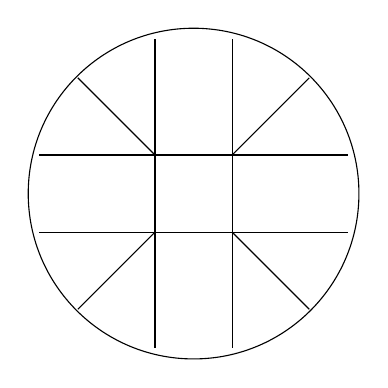
\begin{tikzpicture}[scale=0.7]
		\draw (-2.8,0.7) -- (2.8,0.7);
		\draw (-2.8,-0.7) -- (2.8,-0.7);
		\draw (0.7,-2.8) -- (0.7,2.8);
		\draw (-0.7,-2.8) -- (-0.7,2.8);
		\draw (-2.1,2.1) -- (-0.7,0.7);
		\draw (-2.1,-2.1) -- (-0.7,-0.7);
		\draw (0.7,0.7) -- (2.1,2.1);
		\draw (0.7,-0.7) -- (2.1,-2.1);
		\draw (0,0) circle(3);
	\end{tikzpicture}
	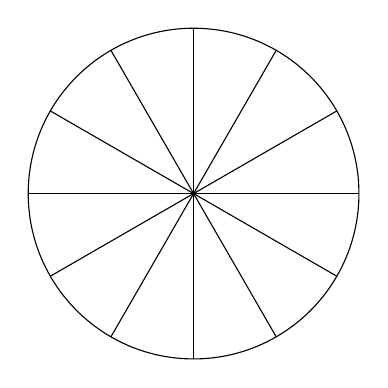
\begin{tikzpicture}[scale=0.7]
		\draw (-3,0) -- (3,0);
		\draw (-3,0) -- (3,0);
		\draw (0,-3) -- (0,2.8);
		\draw (0,-3) -- (0,3);
		\draw (-2.6,-1.5) -- (2.6,1.5);
		\draw (-1.5,-2.6) -- (1.5,2.6);
		\draw (-2.6,1.5) -- (2.6,-1.5);
		\draw (-1.5,2.6) -- (1.5,-2.6);
		\draw (0,0) circle(3);
	\end{tikzpicture}
	\begin{tikzpicture}[scale=0.7]
		\draw (-3,3) -- (3,3);
		\draw (-3,-3) -- (3,-3);
		\draw (-3,-3) -- (-3,3);
		\draw (3,-3) -- (3,3);
		\draw (-1.5,-3) -- (-1.5,3);
		\draw (1.5,-3) -- (1.5,3);
		\draw (-3,-1.5) -- (3,-1.5);
		\draw (-3,1.5) -- (3,1.5);
		\draw (0,-3) -- (0,-1.5);
		\draw (0,1.5) -- (0,3);
		\draw (-3,0) -- (-1.5,0);
		\draw (1.5,0) -- (3,0);
	\end{tikzpicture}
	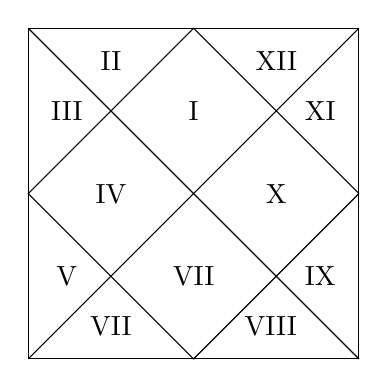
\begin{tikzpicture}[scale=0.7]
		\draw (-3,3) -- (3,3);
		\draw (-3,-3) -- (3,-3);
		\draw (-3,-3) -- (-3,3);
		\draw (3,-3) -- (3,3);
		\draw (-3,-3) -- (3,3);
		\draw (-3,3) -- (3,-3);
		\draw (3,0) -- (0,-3) -- (-3,0) -- (0,3) -- (3,0);

		% подписи
		\draw (-1.5,2.4) node{II};
		\draw (1.5,2.4) node{XII};

		\draw (-2.3,1.5) node{III};
		\draw (0,1.5) node{I};
		\draw (2.3,1.5) node{XI};

		\draw (-1.5,0) node{IV};
		\draw (1.5,0) node{X};

		\draw (-2.3,-1.5) node{V};
		\draw (0,-1.5) node{VII};
		\draw (2.3,-1.5) node{IX};

		\draw (-1.5,-2.4) node{VII};
		\draw (1.4,-2.4) node{VIII};
	\end{tikzpicture}
}

В нашей книге мы будем использовать диаграмму, показанную в последнем примере, которая наиболее популярна в индийской астрологии. Каждый ее сектор представляет дом, который имеет свой номер. Функциональный порядок расположения домов указан на диаграмме от одного до двеннадцати. Он никогда не изменяется, поэтому номера домов в диаграмме цифрами не обозначаются. Цифрами обозначены только знаки Зодиака согласно их порядковому номеру. Знаки зодиака идут в определенной последовательности и имеют свои порядковые номера:


\begin{table}[tph!]
	\centering

	% Расширить по вертикали
	\renewcommand{\arraystretch}{1.5}

	% Заполним данными
	\begin{tabular}{lll}
		1 --- Овен     & 5 --- Лев      & 9 --- Стрелец \\
		2 --- Телец    & 6 --- Дева     & 10 --- Козерог \\
		3 --- Близнецы & 7 --- Весы     & 11 --- Водолей \\
		4 --- Рак      & 8 --- Скорпион & 12 --- Рыбы \\
	\end{tabular}
\end{table}

Так как каждому знаку соответствует определенный номер, то вместо символических обозначений мы будем использовать в диаграмме соответствующие цифры.

В нашем примере восходящим знаком является Водолей, и его номерной знак --- это всегда первый (I) дом, поэтому в секторе, который соответствует первому дому, поставим цифру 11. Во втором (II) доме --- цифру 12, в третьем (III) доме --- цифру 1, в четвертом (IV) доме --- цифру 2, в пятом (V) доме --- цифру 3, в  шестом (VI) доме --- цифру 4, в седьмом (VII) доме --- цифру 5, в восьмом (VIII) доме --- цифру 6, в девятом (IX) доме --- цифру 7, в десятом (X) доме --- цифру 8, в одиннадцатом (XI) доме --- цифру 9 и в двеннадцатом (XII) доме --- цифру 10. Теперь поместим уже расчитанные планеты в сектора, соответствующие номерам знаков Зодиака. В диаграмме это будет выглядеть так:

\natal[asc=11,three=Луна\\Кету,nine=Раху\\Юпитер\\Марс,ten=Солнце\\Сатурн,eleven=Меркурий,twelve=Венера]{}

Это и есть карта рождения, составленная по индийской астрологической системе. Определим, в каких домах находятся планеты:

\begin{mylist}
	\item Луна и Кету --- в 3-м доме.
	\item Юпитер, Раху и Марс --- в 9-м доме.
	\item Солнце и Сатурн --- в 10-м доме.
	\item Меркурий --- в 11-м доме.
	\item Венера --- в 12-м доме.
\end{mylist}

Что означают позиции планет в различных домах, вы узнаете в следующих главах книги.

Индийская астрология --- предсказательная астрология, поэтому вы должны научиться расчитывать периоды жизни, которые связаны с расчетами главных периодов и подпериодов планет.

\subsection{Расчет главных периодов и подпериодов планет}

Мы знаем, что Зодиак разделен на 12 равных знаков. Но в индийской предсказательной астрологии он еще делится на 27 равных частей, которые называются \emph{лунными созвездиями} или \emph{накшатрами}. Координаты лунных созвездий относительно знаков Зодиака даны в таблице~\ref{tbl:nakshatras}. Индийские риши разделили 27 созвездий на 9 групп по 3 созвездия в каждой. Каждая группа имеет своего ``хозяина'' --- одну из девяти планет. Каждая планета оказывает влияние на жизнь человека в определенный период времени.


\begin{table}[tph!]
	\caption{27 лунных созвездий(накшатр)}
	\label{tbl:nakshatras}

	\centering

	% Расширить по вертикали
	\renewcommand{\arraystretch}{1}

	% Заполним данными
	\begin{tabular}{|p{.01\textwidth}p{.18\textwidth}|p{.01\textwidth}p{.18\textwidth}|p{.01\textwidth}p{.21\textwidth}|p{.09\textwidth}|p{.12\textwidth}|}
		\hline
		\multicolumn{6}{|c|}{} & Хозяева & Продол-\\
		\multicolumn{6}{|c|}{Накшатры и их протяженность} & групп созвездий & житель-ность главных периодов \\
		\hline
		1. & Ашвини & 10. & Магха & 19. & Мула & Кету & 7 лет /\\
		& \signum{0}{13}{\aries}--\signum{13}{20}{\aries}& & \signum{0}{13}{\leo}--\signum{13}{20}{\leo} & & \signum{0}{13}{\sagittarius}--\signum{13}{20}{\sagittarius} & & 2520\,дней\\
		& & & & & & & \\

		2. & Бхарани & 11. & Пурва"=Пхалунги & 20. & Пурвашадха & Венера & 20 лет /\\
		& \signum{13}{20}{\aries}--\signum{26}{40}{\aries}& & \signum{13}{20}{\leo}--\signum{26}{40}{\leo} & & \signum{13}{20}{\sagittarius}--\signum{26}{40}{\sagittarius} & & 7200\,дней\\
		& & & & & & & \\

		3. & Криттика & 12. & Уттар"=Пхалунги & 21. & Уттарашадха & Солнце & 6 лет /\\
		& \signum{26}{40}{\aries}--\signum{10}{}{\taurus}& & \signum{26}{40}{\leo}--\signum{10}{}{\virgo} & & \signum{26}{40}{\sagittarius}--\signum{10}{}{\capricornus} & & 2160\,дней\\
		& & & & & & & \\

		4. & Рохини & 13. & Хаста & 22. & Шравана & Луна & 10 лет /\\
		& \signum{10}{}{\taurus}--\signum{23}{20}{\taurus}& & \signum{10}{}{\virgo}--\signum{23}{20}{\virgo} & & \signum{10}{}{\capricornus}--\signum{23}{20}{\capricornus} & & 3600\,дней\\
		& & & & & & & \\

		5. & Мригашира & 14. & Читра & 23. & Дханишта & Марс & 7 лет /\\
		& \signum{23}{20}{\taurus}--\signum{6}{40}{\gemini}& & \signum{23}{20}{\virgo}--\signum{6}{40}{\libra} & & \signum{23}{20}{\capricornus}--\signum{6}{40}{\aquarius} & & 2520\,дней\\
		& & & & & & & \\

		6. & Ардра & 15. & Свати & 24. & Сатабиша & Раху & 18 лет /\\
		& \signum{6}{40}{\gemini}--\signum{20}{}{\gemini}& & \signum{6}{40}{\virgo}--\signum{20}{}{\virgo} & & \signum{6}{40}{\aquarius}--\signum{20}{}{\aquarius} & & 6480\,дней\\
		& & & & & & & \\

		7. & Пунарвасу & 16. & Висакха & 25. & Пурва"=Бхадрапада & Юпитер & 16 лет /\\
		& \signum{20}{}{\gemini}--\signum{3}{20}{\cancer}& & \signum{20}{}{\virgo}--\signum{3}{20}{\scorpio} & & \signum{20}{}{\aquarius}--\signum{3}{20}{\pisces} & & 5760\,дней\\
		& & & & & & & \\

		8. & Пушья & 17. & Анурадха & 26. & Уттар"=Бхадрапада & Сатурн & 19 лет /\\
		& \signum{3}{20}{\cancer}--\signum{16}{40}{\cancer}& & \signum{3}{20}{\scorpio}--\signum{16}{40}{\scorpio} & & \signum{3}{20}{\pisces}--\signum{16}{40}{\pisces} & & 6840\,дней\\
		& & & & & & & \\

		9. & Ашлеша & 18. & Джиешта & 27. & Ревати & Мер- & 17 лет /\\
		& \signum{16}{40}{\cancer}--\signum{0}{}{\leo}& & \signum{16}{40}{\scorpio}--\signum{0}{}{\sagittarius} & & \signum{16}{40}{\pisces}--\signum{0}{}{\aries} & курий & 6120\,дней\\

		\hline
	\end{tabular}
\end{table}

Группы лунных созвездий, их хозяева, главные периоды и подпериоды планет даны в таблице~\ref{tbl:stargroups}

Для определения времени, в котором будут действовать различные главные периоды и подпериоды планет, необходимо знать хозяев лунных созвездий, точные координаты Луны (с точностью до минут) и иметь под рукой таблицу главных периодов и подпериодов планет.

В нашем гороскопе-примере координаты Луны, равны \coord{14}{51}{12} Овна. Округлим до минут и получим \coord{14}{51}{0} Овна.

По таблице~\ref{tbl:nakshatras} определяем, что Луна в момент рождения человека находилась под созвездием Бхарани, границы которого проходят от \coord{13}{20}{0} Овна до \coord{26}{40}{0} Овна. Протяженность каждого созвездия равна \coord{13}{20}{0}, или \(800^\prime\).


\begin{table}[tph!]
	\caption{Подпериоды планет в годах, месяцах, днях}
	\label{tbl:stargroups}

	\centering

	% Расширить по вертикали
	\renewcommand{\arraystretch}{1}

	% Заполним данными
	\begin{tabular}{|p{.1\textwidth}|c|c|c|c|c|c|}
		\hline
		Главные & & & & & & \\
		периоды планет & Солнце & Луна & Марс & Раху & Юпитер & Венера \\
		\hline
		Солнце   & 3м 18д  & 6м     & 4м 6д    & 10м 24д   & 9м 18д    & 11м 12д   \\
		Луна     & 6м      & 10м 9д & 7м       & 1г 6м     & 1г 4м     & 1г 7м     \\
		Марс     & 4м 6д   & 7м     & 4м 27д   & 1г 18д    & 11м 6д    & 1г 1м 9д  \\
		Раху     & 10м 24д & 1г 6м  & 1г 18д   & 2г 8м 12д & 2г 4м 24д & 2г 10м 6д \\
		Юпитер   & 9м 18д  & 1г 4м  & 11м 6д   & 2г 4м 24д & 2г 1м 18д & 2г 6м 12д \\
		Сатурн   & 11м 12д & 1г 7м  & 1г 1м 9д & 2г 10м 6д & 2г 6м 12д & 3г 3д     \\
		Меркурий & 10м 6д  & 1г 5м  & 11м 27д  & 2г 6м 18д & 2г 3м 6д  & 2г 8м 9д  \\
		Кету     & 4м 6д   & 7м     & 4м 27д   & 1г 18д    & 11м 6д    & 1г 1м 9д  \\
		Венера   & 1г      & 1г 8м  & 1г 2м    & 3г        & 2г 8м     & 3г 2м     \\
		\hline
	\end{tabular}
	\newline
	\begin{tabular}{|p{.1\textwidth}|c|c|c|}
		\hline
		Главные & & & \\
		периоды планет & Сатурн & Меркурий & Кету \\
		\hline
		Солнце   & 10м 6д    & 4м 6д    & 1г \\
		Луна     & 1г 5м     & 7м       & 1г 8м \\
		Марс     & 11м 27д   & 4м 27д   & 1г 2м \\
		Раху     & 2г 6м 18д & 1г 18д   & 3г \\
		Юпитер   & 2г 3м 6д  & 11м 6д   & 2г 8м \\
		Сатурн   & 2г 8м 9д  & 1г 1м 9д & 3г 2м \\
		Меркурий & 2г 4м 27д & 11м 27д  & 2г 10м \\
		Кету     & 11м 27д   & 4м 27д   & 1г 2м \\
		Венера   & 2г 10м    & 1г 2м    & 3г 4м \\
		\hline
	\end{tabular}
\end{table}

Из таблицы~\ref{tbl:nakshatras} следует, что хозяином Бхарани является Венера и ее главный период равен 20 годам, или 7200 дням. Если бы, предположим, в момент рождения Луна оказалась в \coord{13}{20}{0} Овна, то человек вступил бы в двадцатилетний главный период Венеры. В нашем примере Луна находилась в \coord{14}{51}{0} Овна, а это значит, что главный период Венеры для данного человека будет неполный. Нам нужно определить какой путь Луна должна пройти, чтобы достичь отметки \coord{26}{40}{0} Овна. Найдем остаточный путь Луны:

\calc{\coord{26}{40}{0} - \coord{14}{51}{0} = \coord{11}{49} = 709^\prime}

Теперь высчитаем, сколько человеку осталось прожить в главном периоде Венеры от своего дня рождения:

\calc{\dfrac{7200}{800^\prime} = 9}

9 --- сколько дней приходится в главном периоде Венеры на одну угловую минуту пути Луны. Зная остаточный путь Луны в угловых минутах (\(709^\prime\)), определим, сколько дней осталось жить в главном периоде Венеры:

\calc{9 * 709^\prime = 6381}

В индийской астрологии используется система, в которой 1 год равен 360 дням и 1 месяц --- 30 дням. Эта система основана на периоде годового обращения Солнца (\(1^\circ\) равен 1 дню).

Для удобства дальнейшего подсчета переводим полученные дни в годы имесяцы:

\calc{\dfrac{6381}{360} = 17:8:21}

В нашем примере человек родился 4 декабря 1957 года. К этой дате рождения прибавим 17 лет 8 месяцев и 21 день и в результате получим дату, до которой будет действовать главный период Венеры. Затем в силу вступит главный период Солнца (6 лет), потом главный период Луны (10 лет), главный период Марса (7 лет), главный период Раху (18 лет), главный период Юпитера (16 лет) и\,т.\,д. В таблице~\ref{tbl:stargroups} вы увидите их последовательность.

После определения дат главных периодов приступим к определению дат подпериодов планет. Главный период Солнца начнется с подпериода Солнца, потом наступит подпериод Луны, подпериод Марса, подпериод Раху, подпериод Юпитера, подпериод Сатурна, подпериод Меркурия, подпериод Кету и последний подпериод Венеры главного периода Солнца. Таким же образом определяются даты подпериодов главного периода Луны, главного периода Марса, главного периода Раху, главного периода Юпитера и\,т.\,д. Для примера дадим даты девяти подпериодов главного периода Солнца:

\begin{table}[tph!]
	\centering

	% Расширить по вертикали
	\renewcommand{\arraystretch}{1.5}

	% Заполним данными
	\begin{tabular}{|lllll|}
		\hline
		гл. период & подпериод & день & месяц & год \\
		\hline
		Солнце & Солнце & 25 & август & 1975 \\
		Солнце & Луна & 13 & декабрь & 1975 \\
		Солнце & Марс & 13 & июнь & 1976 \\
		Солнце & Раху & 19 & октябрь & 1976 \\
		Солнце & Юпитер & 13 & сентябрь & 1977 \\
		Солнце & Сатурн & 1 & июль & 1978 \\
		Солнце & Меркурий & 13 & июнь & 1979 \\
		Солнце & Кету & 19 & апрель & 1980 \\
		Солнце & Венера & 25 & август & 1980 \\
		Луна & Луна & 25& август & 1981 \\
		\hline
	\end{tabular}
\end{table}

После того как вы определите даты подпериодов последующих главных периодов, предлагаемый гороскоп-пример будет приведен в соответствие с периодами жизни.

